This chapter describes specific implementation details of IDDR system.

\section{Overview} 
We implemented the IDDR system based on the Linux kernel, version 3.5.0 and
Xen version 4.2.1. The application domain and the driver domain run the same kernel
binary. Table~\ref{tab:base} summarizes our implementation efforts in
terms of the number of lines of code.

\begin{table}
\caption{Implementation efforts in terms of number of lines of code.}
\begin{center}
\begin{tabular}{lll}
  \hline
  \label{tab:base}
  Component & Interrupt based IDDR & Spinning based IDDR \\
  \hline
  Linux Kernel & 6 & 6\\
  Xen & 252 & 252\\
  Front-end Driver & 611 & 712\\
  Back-end Driver & 692 & 752\\
  \hline 
  Total & 1561 & 1722\\
  \hline
\end{tabular}
\end{center}
\end{table}

The IDDR system implementation did not require any changes to the device
driver code. However, we did make a small number of changes to the Xen
and Linux kernel.

Figure~\ref{fig:Implementation overview} shows the implementation overview of 
the spinning based IDDR system.

\begin{figure}[!ht]
\centering
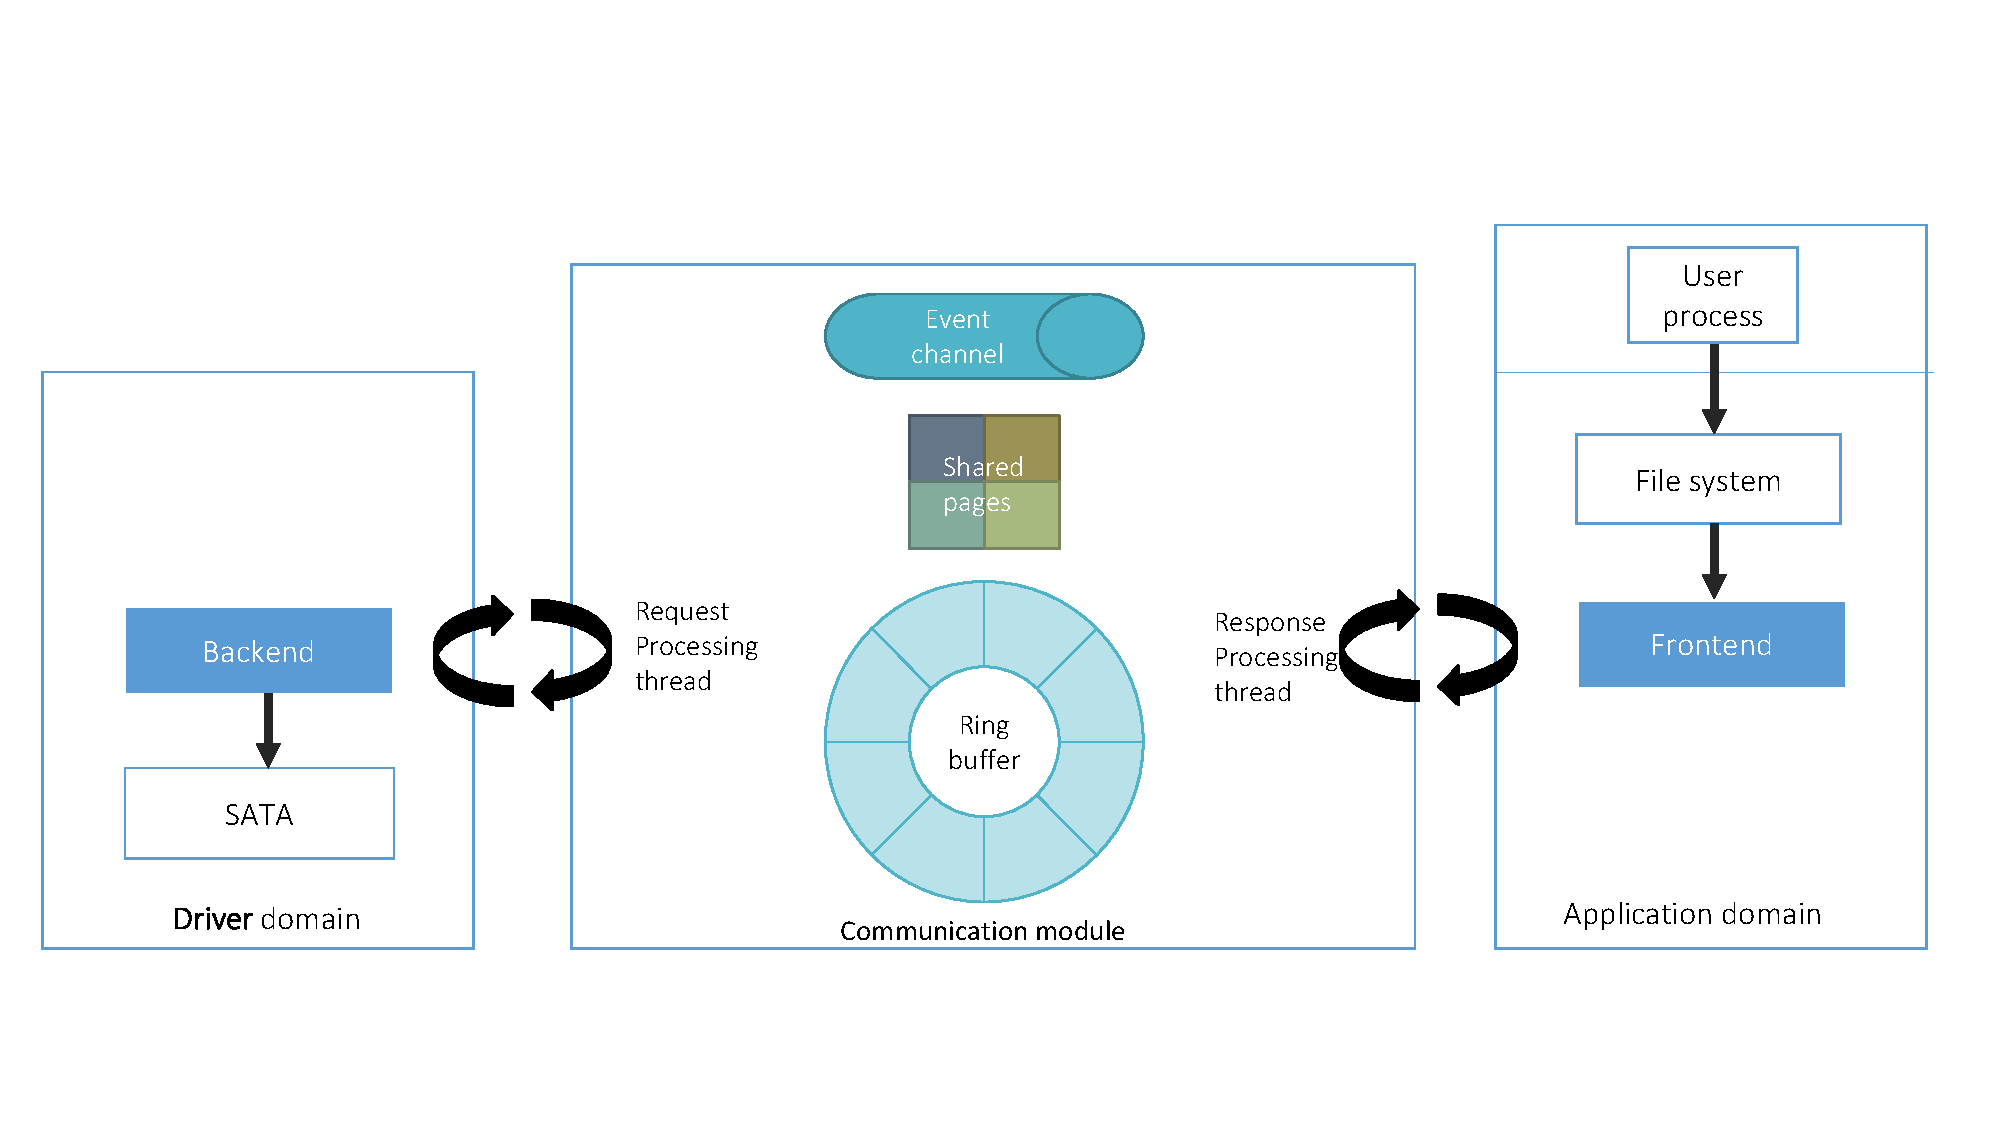
\includegraphics[scale=.5]{impl_overview_new}
\caption{Implementation overview of spinning based IDDR system}
\label{fig:Implementation overview}
\end{figure}

\section{Communication Module}
This section describes the implementation details of the communication
module of interrupt based IDDR system and spinning based IDDR system.

\subsection{Interrupt based IDDR system}
As Section~\ref{sub:communicationmodule} describes, the role of the communication module in interrupt based IDDR system is to:
\begin{enumerate} 
\item Share requests and responses between the driver domain and the application domain
\item Share the data associated with read/write requests/responses
\item Notify the domain upon the availability of requests and responses 
\end{enumerate}
\paragraph{Shared Request and Response Queue:}
In order to implement the first role of the communication module, we
use the ring buffer mechanism provided by Xen. A ring buffer is a shared
I/O ring, which is explained in Section~\ref{subsec:io rings}. We divide
the ring buffer into the front ring and the back ring. The IDDR system
uses the front ring as the shared request queue and the back ring as
the shared response queue. The front ring shares requests and is called
as \textit{shared request queue}. The back ring shares responses and is
called as \textit{shared response queue}.

The IDDR system allocates the ring buffer in the initialization stage
of the communication module and initializes the ring buffer in the
application domain. Whenever the frontend driver receives a request from
an application in the application domain, the frontend driver removes the
request from the device driver queue and submits it to the communication
module. The communication module checks for a free space in the shared
request queue, and if available, it allocates the space for the new
request. After batching requests together, the communication module
pushes all requests to the shared request queue.

\paragraph{Shared Memory for Read/Write Data:}
We use the ring buffer only to share requests and responses. In order
to share data associated with read/write requests/responses we use
shared pages.

As explained in Section~\ref{subsec:sharedpages}, a grant table is used
for sharing memory between domains. We use a grant table to share memory
between the application domain and the driver domain.

\paragraph{Event Notification:}
We create an event channel in the initialization stage of the
communication module in the application domain and connect to it in 
the initialization stage of the communication module
in the driver domain. We attach an interrupt handler routine for the
event channel in both domains. The interrupt handler routine in the 
application domain reads responses from the shared
response queue and forwards them to the frontend driver. The interrupt
handler routine in the driver domain reads requests from the shared
request queue and forwards them to the backend driver.

\subsection{Spinning Based IDDR System}
This section describes the communication module of the spinning based IDDR system:

\subsubsection*{Read response thread in the application domain:} 
In the spinning based IDDR system we create a kernel thread called the \textit{read
response thread} during an initialization stage of the communication
module in the application domain. The \textit{read response thread} spins
to check if responses are available in the shared response queue. If a
response is available, it reads the response from the shared response
queue. However, if a response is not available in the shared response
queue, the thread goes into a sleep state after spinning for threshold time. We
maintain the status of the thread as \texttt{SLEEPING} or \texttt{RUNNING}
in the shared data structure. When the thread reaches threshold time, we change
its state from \texttt{RUNNING} to \texttt{SLEEPING}, and we check again the
response queue for new responses in order to avoid race condition. 

Obviously, a thread shouldn't sleep unless it is assured that somebody else, 
somewhere, will wake it up. The code doing the waking up must also be able to 
identify the thread to be able to do its job. We use a Linux data structure called 
\texttt{wait queue} to find the sleeping thread. 

Wait queue is a list of threads, all waiting for a specific event~\cite{Galvin, Bovet:2005:ULK:1077084}. 
We initialize the wait queue for the read response thread during an initialization stage 
of the communication module in the application domain. The read response thread sleeps 
in the wait queue, waiting for a flag denoting the availability of the response to be set. 
The communication module in the driver domain checks the status of the read response 
thread after pushing responses on the shared response queue. If the status is 
\texttt{SLEEPING} then it sends a virtual interrupt. It uses an event channel to wake the \textit{read
response thread}. The wake up signal is sent in the form of an event channel notification from the driver
domain to the application domain. 

Similar to interrupt based IDDR system, we create a new event channel in
the initialization stage of the communication module in the application
domain. We attach an interrupt handler routine for the event channel
in the application domain. In the interrupt handler, the communication
module wakes up the read response thread if it is sleeping.

\subsubsection*{Read request thread in the driver domain:}
The implementation of the \textit{read request thread} is basically 
the same as the \textit{read response thread}. The \textit{read request thread}
spins in the driver domain for requests to be available in the request queue.


\section{Application Domain}

\subsection{Frontend Driver}
\subsubsection*{Interrupt based IDDR System}
The core responsibility of the frontend driver in interrupt based IDDR system is to:
\begin{enumerate}
\item Provide an interface which appears as a block device to file systems/ user applications.
\item Accept a request from file system or a user application
\item Send the request to the driver domain
\item Send a completion notification to a user application after reading the response
\end{enumerate}

The implementation of the frontend driver is split into 3 phases: 
\begin{enumerate}
\item Initialization
\item Submit request to the communication module
\item Send a completion notification to a user application
\end{enumerate}

\paragraph{Initialization}
During the initialization phase, the frontend driver creates a separate
interface for each block device. The interface for each block device is
associated with a device driver queue. Read and write requests issued
on the interface are queued in this device driver queue.

\paragraph{Dequeue and Submit Request:}
The frontend driver removes the request submitted to the driver
interface and converts the request into a request structure, which is
required by the backend driver. The request structure points to
the shared memory allocated for the read/write data by the communication
module. The frontend driver then forwards the newly created request
to the communication module, which submits the request to the
backend driver.

\paragraph{Send a request completion notification:}
We maintain a shadow table of all requests which were received in the
device driver queue. The shadow table is a table which contains an entry
of all the requests received. We implement the shadow table as a circular
array of the requests. We maintain an ID for each request. The backend
driver copies this ID into the corresponding response. The ID is used
for mapping the response to the request in the shadow table. When a
response is read by the communication module, it forwards the response
to the frontend driver. The frontend driver searches the corresponding
request in the shadow table, and sends a completion notification to 
an user application.

\subsubsection*{Spinning Based IDDR System}
The core responsibility and implementation of the frontend driver of 
the spinning based IDDR system is similar to the interrupt based IDDR system.

\section{Driver Domain}

\subsection{Backend Driver}

The role of the backend driver in the IDDR system is to:
\begin{enumerate}
\item Read a request through the communication module and convert it to a block I/O request
\item Accept a response from the block device driver
\item Forward the response to the communication module
\end{enumerate}

The implementation of the backend driver is split into 2 phases. 
\begin{enumerate}
\item Convert a request to block I/O request. 
\item Make a response.
\end{enumerate}

\subsubsection*{Convert a Request to Block I/O}
\label{subsec:createbio}
The backend driver converts a request that is shared through the
communication module into a block I/O request, so that the block device
understands the request. In order to create a block I/O request, pages from
the shared memory are mapped and inserted into the block I/O request structure and
required information is copied from the shared request into the block I/O
structure. The newly created request is sent to the lower layer for execution. 
Once the block I/O request execution is completed, the system calls a callback function.

\subsubsection*{Make a Response and Enqueue}
Irrespective of the success or failure of execution of a request,
the backend driver makes a response in the callback function. In this
callback function, the result of execution and a request ID is
copied into a newly allocated response structure. The request ID is used
as an index in the shadow table to map a response to a request. The
communication module pushes the response into the shared response queue, 
so that the response is made available to the application domain.

